\section{Exercício 1}

Considere o experimento computacional denominado “Polynomial Curve Fitting”, usado
diversas vezes no livro texto (veja páginas 4 e 5 do livro, bem como Apêndice A), considerando a
ordem do modelo sendo M = 9 e o tamanho da amostra sendo N = 10.
Faça:

\begin{enumerate}[label=(\alph*)]
    \item Calcule a solução de mínimos quadrados (LS) \( \mathbf{w_{LS}} \);
    \item Calcule a solução via regressão ridge (escolha um fator de regularização razoável) \( \mathbf{w_{ridge}} \);
    \item Calcule a solução via regressão lasso (escolha um fator de regularização razoável) \( \mathbf{w_{lasso}} \);
    \item Monte uma tabela exibindo os 10 coeficientes \( \mathbf{w} \) para as 3 soluções obtidas nos itens acima e comente/compare os resultados;
    \item Plote uma figura contendo o processo gerador em verde (a senoide), e suas estimativas \( y_{LS} \), \( y_{ridge} \), e \( y_{lasso} \) em preto, azul e vermelho, respectivamente;
    \item Repita todos os itens anteriores para \( N=20 \) e \( N=50 \).
\end{enumerate}

\subsection{Resposta do item (a)}
Para responder esse item foi utilizada a classe $LinearRegression()$ da biblioteca \textit{sklearn} para linguagem \textit{Python}, que realiza uma regressão linear utilizando mínimos quadrados. Foi escolhido um polinômio de ordem 9 como modelo.
\begin{figure}[H]
    \centering
    \caption{Solução para mínimos quadrados (LS)}
    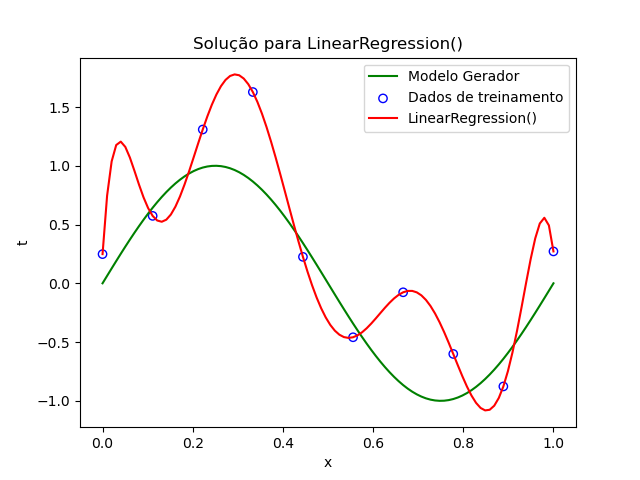
\includegraphics[width=12cm]{E1_a.png}
\end{figure}
A regressão linear por mínimos quadrados não introduz nenhuma regularização e por isso a curva vermelha passa exatamente pelos dados de treinamento, mostrando que eles foram decorados overfitting.


\subsection{Resposta do item (b)}
Para responder esse item foi utilizada a classe $Ridge()$ da biblioteca \textit{sklearn} para linguagem \textit{Python}, que realiza uma regressão linear utilizando mínimos quadrados e regularização de norma $L_2$ (Ridge). Foi escolhido um polinômio de ordem 9 como modelo e o fator de regularização $\lambda$, que na classe $Ridge()$ é chamado de \textit{alpha}, que melhor adaptou a curva ao modelo gerador foi $1^{-0.5}$.
\begin{figure}[H]
    \centering
    \caption{Solução para Ridge com $\lambda = 1^{-0.5}$}
    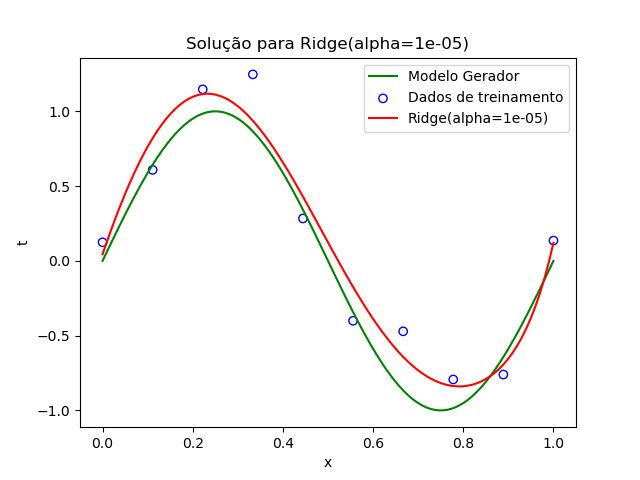
\includegraphics[width=12cm]{E1_b.png}
\end{figure}
A regressão Ridge introduz uma penalização nos coeficientes através do fator de regularização, ajudando a evitar overfitting.

\subsection{Resposta do item (c)}
Para responder esse item foi utilizada a classe $Lasso()$ da biblioteca \textit{sklearn} para linguagem \textit{Python}, que realiza uma regressão linear utilizando mínimos quadrados e regularização de norma $L_1$ (Lasso). Foi escolhido um polinômio de ordem 9 como modelo e o fator de regularização $\lambda$, que na classe $Lasso()$ é chamado de \textit{alpha}, que melhor adaptou a curva ao modelo gerador foi $1^{-0.5}$.
\begin{figure}[H]
    \centering
    \caption{Solução para Lasso com $\lambda = 10^{-0.6}$}
    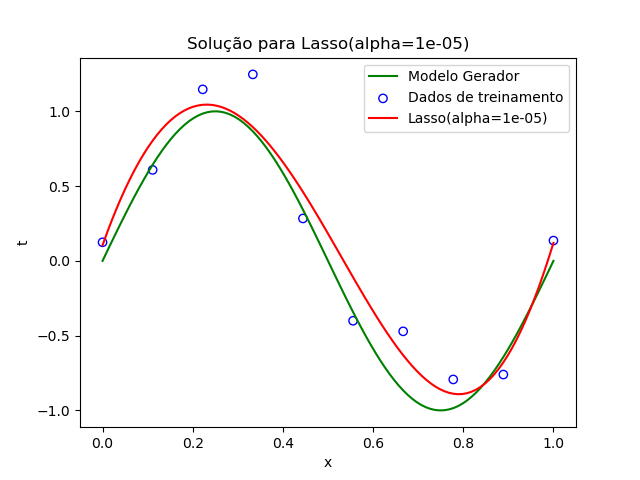
\includegraphics[width=12cm]{E1_c.png}
\end{figure}
A regressão Lasso, assim como a Ridge, introduz uma penalização nos coeficientes através do fator de regularização, ajudando a evitar overfitting.

\subsection{Resposta do item (d)}

A tabela abaixo exibindo os coeficientes para as três soluções permite comparar diretamente o impacto da regularização nos coeficientes.

\begin{table}[H]
\caption{Coeficientes para $N=10$}
\resizebox{\textwidth}{!}{
\begin{tabular}{lllllllllll}
    \toprule
    Modelo & w0 & w1 & w2 & w3 & w4 & w5 & w6 & w7 & w8 & w9 \\
    \midrule
    LS & 0.00 & 33.81 & -652.62 & 5410.54 & -21973.73 & 48026.65 & -58345.99 & 37810.21 & -10973.23 & 664.37 \\     
    Ridge & 0.00 & 8.87 & -14.84 & -21.96 & 25.51 & 24.50 & -3.61 & -23.28 & -16.17 & 21.04 \\
    Lasso & 0.00 & 8.50 & -20.39 & 3.66 & 5.68 & 3.20 & 0.97 & -0.19 & -0.66 & -0.76 \\
    \bottomrule
\end{tabular}
}
\end{table}

A regressão por mínimos quadrados sem regularização tende a produzir coeficientes maiores, um dos sinais que indicam overfitting ou pelo menos uma alta sensibilidade aos altos de treinamento. Enquanto que os coeficientes produzidos pela Ridge e pela Lasso são menores.

Além disso, é possível observar a presença de alguns coeficientes praticamente nulos para a Lasso. Esse resultado era esperado, uma vez que a Lasso, por utilizar a norma $L_1$, tende a produzir uma seleção mais esparsa, selecionando atributos mais importantes.

Enquanto isso, a regressão Ridge, apesar de não selecionar atributos como a Lasso, tende a penalizar, e consequentemente reduzir, ainda mais os coeficientes grandes.



\subsection{Resposta do item (e)}
\begin{figure}[H]
    \centering
    \caption{Comparação entre as soluções para $N=10$}
    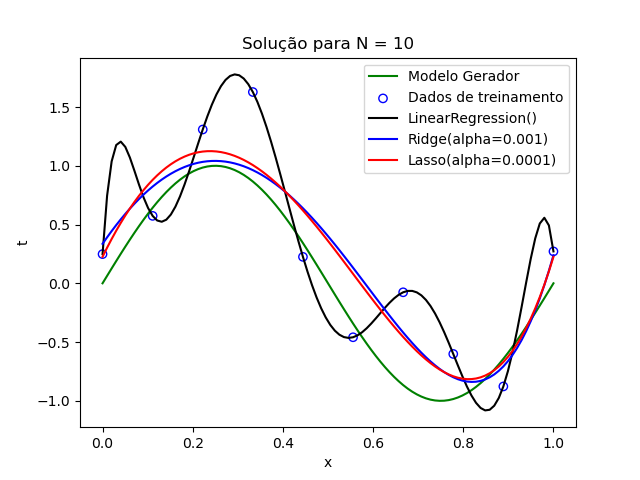
\includegraphics[width=12cm]{E1_e.png}
\end{figure}

\subsection{Resposta do item (f)}

\begin{figure}[H]
    \centering
    \caption{Comparação entre as soluções para $N=20$}
    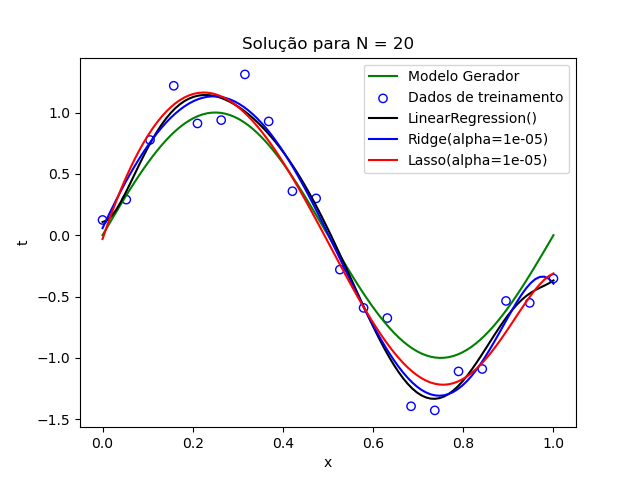
\includegraphics[width=12cm]{E1_f20.png}
\end{figure}
\begin{table}[H]
    \caption{Coeficientes para $N=20$}
    \resizebox{\textwidth}{!}{
        \begin{tabular}{lllllllllll}
            \toprule
            Modelo & w0 & w1 & w2 & w3 & w4 & w5 & w6 & w7 & w8 & w9 \\
            \midrule
            LS & 0.00 & 0.13 & 133.29 & -1042.60 & 3592.94 & -6598.01 & 6040.15 & -1620.50 & -1137.52 & 631.65 \\
            Ridge & 0.00 & 7.94 & -10.61 & -17.66 & 2.91 & 14.55 & 13.52 & 4.83 & -5.11 & -10.82 \\
            Lasso & 0.00 & 11.00 & -26.25 & 2.05 & 8.34 & 7.01 & 3.69 & 0.35 & -2.11 & -4.36 \\
            \bottomrule
        \end{tabular}
    }
\end{table}

\begin{figure}[H]
    \centering
    \caption{Comparação entre as soluções para $N=50$}
    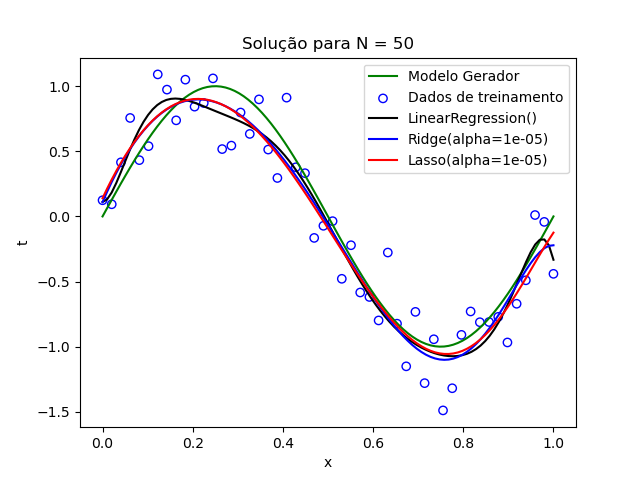
\includegraphics[width=12cm]{E1_f50.png}
\end{figure}
\begin{table}[H]
    \caption{Coeficientes para $N=50$}
    \resizebox{\textwidth}{!}{
    \begin{tabular}{lllllllllll}
        \toprule
        Modelo & w0 & w1 & w2 & w3 & w4 & w5 & w6 & w7 & w8 & w9 \\
        \midrule
        LS & 0.00 & -0.06 & 228.03 & -2656.39 & 13838.07 & -40023.24 & 67930.77 & -67287.01 & 36037.64 & -8068.26 \\    
        Ridge & 0.00 & 8.06 & -23.82 & 17.17 & -5.30 & -8.80 & 5.11 & 16.26 & 10.42 & -19.44 \\
        Lasso & 0.00 & 7.42 & -18.67 & 1.59 & 5.49 & 4.71 & 2.67 & 0.51 & -1.09 & -2.90 \\
        \bottomrule
    \end{tabular}
    }
\end{table}






